% =============================================================================
% Integrantes: Arthur Meneses Neves, Danilo Oliveira Santos, Matheus Gabriel
% Viana Araujo, João Victor Vidal Barbosa, Guilherme Araujo Castro
%
% Síntese: Artigo parcial (Parte 2 / N1) do projeto da disciplina de
% Inteligência Artificial, no template SBC. Descreve o problema (classificar
% o capítulo CID-10 da causa básica de óbito a partir de atributos
% sociodemográficos do SIM, 2000-2026, Brasil), a fundamentação teórica e os
% trabalhos relacionados, a metodologia (divisão estratificada, pesos
% balanceados, prevenção de vazamento de rótulo, F1-macro / recall por classe
% / matriz de confusão), o dataset com sua análise exploratória e preparação,
% os aspectos éticos (LGPD, CEP) e os resultados parciais comparando um
% baseline de classe majoritária, Random Forest e XGBoost. Todos os números
% citados vêm das saídas executadas dos notebooks 01, 02 e 03.
%
% Changelog:
%   2026-09-24 — Matheus Araujo — criação do artigo parcial (SBC)
%   2026-09-24 — Matheus Araujo — revisão 1: ajustes de layout (bloco de
%     autores, endereço e Tabela 4 dentro da largura do texto), babel
%     brazilian, distinção entre weighted quantile sketch e tree_method
%     "hist", expectativas apresentadas como plausíveis e não como
%     pré-registradas, argumento do CEP apoiado nos critérios da norma, e
%     nota sobre o intervalo do título do conjunto no portal
% =============================================================================

\documentclass[12pt]{article}

\usepackage{sbc-template}
\usepackage{graphicx,url}
\usepackage[utf8]{inputenc}
\usepackage[brazilian]{babel}

\sloppy

\title{Classificação da causa básica de óbito:\\
  uma comparação entre Random Forest e XGBoost}

\author{Arthur Meneses Neves (10425727), Danilo Oliveira Santos (10410905),\\
  Guilherme Araujo Castro (10427775), João Victor Vidal Barbosa (10410165),\\
  Matheus Gabriel Viana Araujo (10420444)}

\address{Faculdade de Computação e Informática (FCI)\\
Universidade Presbiteriana Mackenzie (UPM)\\
  São Paulo - SP - Brasil
\email{\{10425727,10410905,10427775,10410165,10420444\}@mackenzista.com.br}
}

\begin{document}

\maketitle

\begin{resumo}
  Este artigo relata os resultados do primeiro bimestre de um projeto de IA aplicada que classifica a causa básica de óbito, agregada em seu capítulo da CID-10, a partir de cinco atributos sociodemográficos registrados no Sistema de Informação sobre Mortalidade (SIM): idade, sexo, raça/cor, escolaridade e unidade da federação de residência. O recorte é o Brasil inteiro entre 2000 e 2026 (32.531.918 registros após a preparação, 19 capítulos CID-10 observados). Random Forest e XGBoost, treinados com pesos de amostra balanceados sobre uma divisão estratificada 80/20, são comparados a um baseline de classe majoritária por F1-macro, recall por classe e matrizes de confusão. O XGBoost alcança F1-macro de 0,1406 e o Random Forest 0,1329, contra 0,0224 do baseline; o desempenho absoluto é baixo, o que interpretamos como evidência de que atributos sociodemográficos isolados carregam pouco sinal sobre a causa do óbito. Descrevemos também a análise exploratória, a preparação dos dados, a prevenção explícita de vazamento de rótulo e as considerações éticas e legais da abordagem.
\end{resumo}

\section{Introdução}

\subsection{Contextualização}

O Sistema de Informação sobre Mortalidade (SIM) é o sistema do Ministério da Saúde que consolida as Declarações de Óbito emitidas no país. Seus microdados individuais estão disponíveis desde 1996, obtidos do DATASUS e publicados como dados abertos~\cite{pcdas_sim,sim_dadosgov}. Cada registro traz, além da causa
básica do óbito codificada segundo a Classificação Internacional de Doenças, 10ª revisão (CID-10)~\cite{who_cid10}, atributos sociodemográficos do falecido e dados de residência e ocorrência.

A CID-10 organiza os códigos individuais em capítulos, que agrupam causas afins: doenças do aparelho circulatório, neoplasias, causas externas, e assim por diante. Trabalhar no nível de capítulo transforma a tarefa em um problema com poucas dezenas de classes, tratável com os algoritmos de aprendizado supervisionado vistos na disciplina. Este projeto trabalha com o recorte Brasil, âmbito nacional, período de 2000 a 2026.

\subsection{Justificativa}

Entender como fatores sociodemográficos se relacionam à categoria da causa de óbito é relevante para o planejamento de políticas públicas de saúde. O tema se alinha diretamente ao Objetivo de Desenvolvimento Sustentável 3 (Saúde e Bem-Estar), cuja meta 3.4 prevê reduzir
em um terço, até 2030, a mortalidade prematura por doenças não
transmissíveis~\cite{ods3}.

Fora isso, há também uma justificativa metodológica. O SIM é uma base grande, pública e heterogênea entre anos, e a própria literatura registra limitações persistentes na qualidade do preenchimento das declarações de óbito~\cite{morais2017}. Medir quanto sinal existe apenas nos atributos sociodemográficos, e reportar honestamente esse limite, é um resultado útil por si só, porque delimita o que se pode e o que não se pode esperar de modelos construídos sobre esse subconjunto de variáveis.

\subsection{Motivação}

A motivação do grupo para este tema combina três fatores. Primeiro, o
interesse em aplicar as técnicas de aprendizado de máquina da disciplina a um problema de saúde pública com impacto social claro. Segundo, a disponibilidade de uma base pública, gratuita e de escala real, cujo volume obriga o grupo a lidar com questões práticas de engenharia de dados. Terceiro, o fato de a tarefa ser de desfecho incerto: não sabíamos, ao propor o projeto, quanto da causa de óbito seria previsível a partir de variáveis
sociodemográficas.

\subsection{Objetivo}

Especificamente, o objetivo é classificar a causa básica de óbito, agregada em seu capítulo da CID-10, a partir de atributos sociodemográficos registrados no SIM. Explicitamente:

\begin{itemize}
  \item Variáveis de entrada (atributos): idade em anos completos (numérica), sexo (masculino, feminino), raça/cor autodeclarada (branca, preta, amarela, parda, indígena, ignorado), escolaridade (nenhuma, 1 a 3 anos, 4 a 7 anos, 8 a 11 anos, 12 anos ou mais, ignorado) e unidade da federação de residência, derivada do código do município de residência (27 categorias). São cinco variáveis.
  \item Variável de saída (classes): o capítulo da CID-10 da causa básica, com $k = 19$ classes efetivamente observadas nos dados (capítulos I a XVIII e XX; os capítulos XIX e XXI nunca ocorrem como causa básica nesta base). A lista completa das classes e sua frequência estão na
    Tabela~\ref{tab:classes}.
  \item Período: 2000 a 2026, sendo 2026 um ano parcial.
  \item Região: Brasil, âmbito nacional, sem recorte por estado ou região.
\end{itemize}

Nenhuma variável que descreva a cadeia de causas da própria declaração de
óbito  é usada como entrada, para evitar vazamento do rótulo;
a Seção~\ref{sec:metodologia} detalha como isso é garantido e verificado em código.

\subsection{Contribuições esperadas}

Uma análise exploratória documentada e reprodutível do SIM 2000-2026, incluindo as inconsistências de formato entre anos e a evolução do não-preenchimento de raça/cor e escolaridade.

Uma comparação entre um baseline de classe majoritária, Random Forest e XGBoost para essa tarefa, com discussão explícita de desempenho por classe, custo computacional, desbalanceamento e limitações.

Uma medida empírica de quanto sinal sobre a causa de óbito existe apenas em atributos sociodemográficos, reportada sem superestimação.

\section{Fundamentação Teórica e Trabalhos Relacionados}

\subsection{Conceitos fundamentais}

O problema tratado é de classificação supervisionada multiclasse, em que, dado um vetor de atributos $x$, atribuir a ele um rótulo $y$ entre $k$ classes mutuamente exclusivas, aprendendo a associação a partir de exemplos rotulados. Os dois algoritmos comparados pertencem à família dos \emph{ensembles} de árvores de decisão.

Random Forest~\cite{breiman2001} treina um conjunto de árvores de decisão, cada uma sobre uma amostra bootstrap dos dados e com uma seleção aleatória de atributos em cada nó; a predição final é o voto da maioria. A aleatorização reduz a correlação entre as árvores, e o erro de generalização da floresta depende da força das árvores individuais e dessa correlação. É um método robusto a atributos irrelevantes e de treino naturalmente paralelizável.

XGBoost~\cite{chen2016} implementa \emph{gradient boosting}: as
árvores são construídas em sequência, cada uma ajustada ao erro residual das anteriores, com regularização explícita da complexidade. O trabalho original descreve um algoritmo consciente de esparsidade, para dados esparsos, e um esquema aproximado de busca de pontos de corte baseado em quantis ponderados (\emph{weighted quantile sketch}), além de otimizações de acesso a cache, compressão e particionamento dos dados, o conjunto dessas técnicas é o que torna o método viável em bases com dezenas de milhões de linhas, como a nossa. 

Dois conceitos adicionais estruturam a metodologia. O primeiro é o
desbalanceamento de classes: quando uma classe domina a base, a
acurácia deixa de ser informativa, porque um classificador trivial que sempre prevê a classe majoritária já a maximiza. Por isso adotamos o
F1-macro, que é a média aritmética simples do F1 de cada classe e, portanto, dá o mesmo peso a um capítulo com 8,8 milhões de registros e a um com 629, além do recall por classe e da matriz de confusão. O segundo é o vazamento de rótulo (\emph{label leakage}): a presença, entre os atributos, de informação que só existe porque o rótulo já é conhecido. Em uma base de declarações de óbito o risco é concreto, já que os campos de descrição da cadeia de causas são, na prática, o próprio rótulo em outra forma.

A implementação usa a biblioteca scikit-learn~\cite{pedregosa2011} (versão 1.9.1) para o baseline, o Random Forest, a codificação dos atributos, a divisão estratificada e as métricas, e a biblioteca XGBoost (versão 3.4.1) para o \emph{gradient boosting}.

\subsection{Trabalhos relacionados}

Em relação à classificação da causa de óbito em CID-10 a partir de laudos, \cite{mujtaba2017} classificaram automaticamente a causa de óbito em 9 categorias da CID-10 a partir do texto livre de 2.200 laudos de necropsia relacionados a acidentes. Compararam cinco classificadores (Naive Bayes, SVM, k-NN, J48 e Random Forest) combinados com seis estratégias de seleção de atributos; a melhor solução foi o Random Forest com seleção de atributos guiada por especialistas, atingindo cerca de 90\% de acurácia e de F-medida macro com 30 atributos. O contraste com o nosso trabalho é instrutivo e orientou uma decisão metodológica: o alto desempenho ali vem de entradas que \emph{descrevem clinicamente o óbito} (exame externo, lesões, exame interno, histórico médico).  Ou seja, os dois trabalhos resolvem problemas diferentes: lá, automatizar a codificação a partir da descrição clínica; aqui, medir a associação entre perfil sociodemográfico e categoria de causa.

Aprendizado de máquina sobre desfechos de óbito no Brasil.
\cite{silva2022} compararam Regressão Logística, Árvore de Decisão e
Random Forest para prever óbito por COVID-19 a partir de dados clínicos de 134.639 pacientes do SUS atendidos entre janeiro e setembro de 2021. A melhor solução foi o Random Forest, com 77\% de acurácia e AUC-ROC de 0,75, tendo suporte ventilatório, internação em UTI, idade e comorbidades como fatores mais importantes. \cite{santos2019} aplicaram cinco algoritmos (regressão logística, regressão logística penalizada, redes neurais, \emph{gradient boosted trees} e Random Forest) a 2.808 idosos do estudo SABE, em São Paulo, para predizer óbito em cinco anos a partir de 37 preditores demográficos, socioeconômicos e de saúde; todos os modelos superaram AUC-ROC de 0,70, com melhor resultado para redes neurais e regressão logística penalizada. Os dois trabalhos são binários (o óbito ocorre ou não) e contam com preditores clínicos, enquanto o nosso é multiclasse com 19 categorias e usa apenas cinco variáveis sociodemográficas, o que ajuda a dimensionar por que o nosso desempenho absoluto é bem menor. Deles retiramos duas decisões: comparar mais de um algoritmo sob o mesmo protocolo, em vez de reportar um modelo isolado, e relatar métricas que não dependam apenas da
acurácia.

No que diz respeito à qualidade da informação no SIM, \cite{morais2017} avaliaram o próprio SIM como sistema de informação, a partir de 45 indicadores de qualidade aplicados a profissionais e gestores de saúde no nordeste do estado de São Paulo. Embora 31 indicadores tenham recebido avaliação positiva, cerca de 47\% dos usuários relataram algum grau de informação incorreta, especialmente na causa de óbito registrada na declaração, além de problemas de integração com outros sistemas. Esse achado sustenta uma escolha nossa de preparação de dados: tratar os códigos de ``ignorado'' como uma categoria explícita em vez de imputá-los, já que o não-preenchimento é um fenômeno real e sistemático da base, e escondê-lo por imputação estatística mascararia um viés conhecido.

Quanto à lacuna, nenhum dos trabalhos acima classifica a categoria da causa entre óbitos já registrados usando somente atributos sociodemográficos do SIM em escala nacional e em série
histórica longa. É essa combinação que caracteriza a contribuição deste projeto. A comparação contra um baseline de classe majoritária é necessária precisamente porque, com 27\% dos óbitos concentrados em um único capítulo, qualquer métrica global pode parecer razoável sem que o modelo tenha aprendido nada de útil.

\section{Metodologia e Resultados Esperados}
\label{sec:metodologia}

\subsection{Abordagem e etapas}

A solução foi desenvolvida em Python, organizada em três notebooks
(\texttt{01\_eda\_exploratoria.ipynb}, \texttt{02\_preparacao\_dados.ipynb} e
\texttt{03\_resultados\_parciais.ipynb}) e um módulo de funções
(\texttt{src/sim\_utils.py}) coberto por testes automatizados. As etapas são:

\begin{enumerate}
  \item Análise exploratória (notebook 01): distribuições
    demográficas, distribuição e tendência dos capítulos CID-10, sazonalidade e perfil de valores ausentes por ano.
  \item Preparação (notebook 02): decodificação da idade,
    harmonização de escolaridade e raça/cor, derivação da UF a partir do
    município, derivação do alvo (capítulo CID-10) e aplicação dos filtros,
    com contabilidade de linhas descartadas em cada etapa.
  \item Definição do protocolo de avaliação antes do treino: divisão
    estratificada, tratamento do desbalanceamento, métricas e verificação de
    ausência de vazamento (detalhados abaixo).
  \item Treino e avaliação (notebook 03) do baseline, do Random
    Forest e do XGBoost, sobre o mesmo conjunto de treino e o mesmo conjunto
    de teste, seguidos de uma checagem suplementar de generalização temporal.
\end{enumerate}

O protocolo principal para a divisão treino/teste é uma divisão aleatória estratificada por classe, 80\% para treino e 20\% para teste. 

Adotamos pesos de amostra balanceados iguais para Random Forest e XGBoost. Os pesos vão de 0,1948 (capítulo IX, o majoritário) a 2.723,19 (capítulo VII, o minoritário), razão de 13.977. Essa escolha sacrifica a acurácia nas classes frequentes em troca de recall nas raras, e por isso a acurácia entra no artigo apenas como referência, nunca como critério de
sucesso.

O critério principal para a métrica é o F1-macro. Reportamos também o recall por classe para todas as 19 classes e a matriz de confusão normalizada por linha (em que a diagonal é o recall), além da acurácia e do recall macro como referências, e do tempo de treino de cada modelo como medida de custo computacional.

A prevenção  de vazamento de rótulo é estrutural e verificada. Estrutural, porque a leitura dos CSVs carrega apenas 8 colunas de modo que os campos da cadeia de causas nunca entram em memória, ainda que existam nos arquivos originais. Verificada, porque o notebook de modelagem contém asserções que falham se alguma entrada for o rótulo.


Dado o conjunto restrito de atributos, era plausível esperar desempenho modesto em termos absolutos, mas claramente superior ao baseline em F1-macro, com acerto melhor nos capítulos fortemente associados a idade e sexo (gravidez e parto; afecções perinatais; causas externas) e acerto fraco nas causas de adultos e idosos, que competem entre si no mesmo perfil demográfico. A Seção~\ref{sec:resultados} mostra que foi isso
o que ocorreu.

\subsection{Dataset}
\label{sec:dataset}

A origem representa arquivos ``Mortalidade Geral'' do SIM, mantido
pelo Ministério da Saúde, obtidos no Portal Brasileiro de Dados Abertos em \url{https://dados.gov.br/dados/conjuntos-dados/sim-1979-2019}~\cite{sim_dadosgov}. Os arquivos efetivamente baixados e usados aqui cobrem 2000-2026, conforme registrado em \texttt{data/README.md}. Formato CSV separado por ponto e vírgula, codificação \texttt{latin1}, um arquivo por ano. O diretório \texttt{data/} contém um \texttt{README.md} com a origem, o procedimento de download e a descrição das colunas, conforme orienta o próprio enunciado do
projeto.

Cada registro corresponde a uma Declaração de Óbito. O número de colunas cresce de 39 (2000) para 88 (2024) ao longo da série, conforme o SIM incorporou novos campos. Este projeto lê 8 colunas, presentes
com o mesmo nome em todos os anos conferidos, listadas na Tabela~\ref{tab:colunas}.

\begin{table}[ht]
\centering
\caption{Colunas lidas dos arquivos brutos e seu papel no projeto.}
\label{tab:colunas}
\begin{tabular}{|l|l|l|}
\hline
\textbf{Coluna} & \textbf{Significado} & \textbf{Papel} \\
\hline
\texttt{IDADE} & Idade codificada (unidade + valor) & Entrada (decodificada em anos) \\
\texttt{SEXO} & 0 ignorado, 1 masculino, 2 feminino & Entrada \\
\texttt{RACACOR} & Raça/cor autodeclarada (1 a 5) & Entrada \\
\texttt{ESC} & Escolaridade (1 a 5, 9 ignorado) & Entrada \\
\texttt{CODMUNRES} & Município de residência (IBGE) & Entrada (agregada em UF) \\
\texttt{CAUSABAS} & Causa básica do óbito (CID-10) & Rótulo (capítulo) \\
\texttt{DTOBITO} & Data do óbito & Só análise exploratória \\
\texttt{TIPOBITO} & 1 fetal, 2 não fetal & Só verificação \\
\hline
\end{tabular}
\end{table}

A análise exploratória (notebook 01) revelou problemas de qualidade que definiram a preparação, como, formatos divergentes entre anos, dois tipos de ``sem informação'', não-preenchimento que muda muito ao longo do tempo e mudança na composição das causas.

\begin{figure}[ht]
\centering
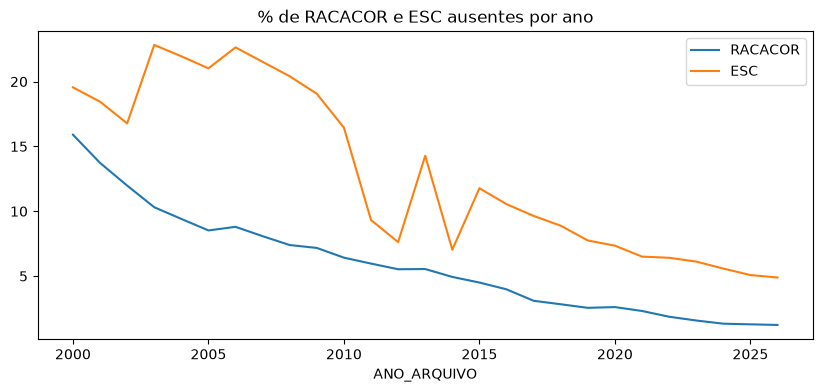
\includegraphics[width=0.95\textwidth]{figuras/ausentes_por_ano.png}
\caption{Percentual de registros com \texttt{RACACOR} e \texttt{ESC} ausentes, por ano (2000-2026). O código 9 (``ignorado''), que é um valor preenchido, não aparece nesta contagem e é tratado à parte.}
\label{fig:ausentes}
\end{figure}

A preparação é feita por uma única função, compartilhada por todos os notebooks, e seu resultado é armazenado em cache (Parquet) cuja chave inclui o tamanho e a data de modificação de cada CSV e uma constante de versão, de modo que um cache desatualizado nunca é usado silenciosamente. As decisões foram:

A Tabela~\ref{tab:classes} e a Figura~\ref{fig:distribuicao} mostram as 19 classes. O capítulo IX (doenças do aparelho circulatório) concentra 27,0141\% dos registros, e o capítulo VII (doenças do olho e anexos), 0,0019\%, uma razão de 13.972 entre o maior e o menor. Cinco capítulos ficam abaixo de 0,5\% dos registros. É esse quadro que justifica as escolhas metodológicas: com 19 classes e essa razão de desbalanceamento, são necessários um baseline explícito, pesos balanceados e métricas macro-agregadas para que o resultado signifique alguma coisa.

\begin{table}[ht]
\centering
\caption{Distribuição do alvo: capítulos da CID-10 observados em 32.531.918 registros (SIM, Brasil, 2000-2026).}
\label{tab:classes}
\begin{tabular}{|l|l|r|r|}
\hline
\textbf{Cap.} & \textbf{Descrição} & \textbf{Registros} & \textbf{\%} \\
\hline
IX    & Doenças do aparelho circulatório                       & 8.788.199 & 27,0141 \\
II    & Neoplasias (tumores)                                   & 5.108.490 & 15,7030 \\
XX    & Causas externas de morbidade e mortalidade             & 3.712.335 & 11,4114 \\
X     & Doenças do aparelho respiratório                       & 3.516.512 & 10,8094 \\
XVIII & Sintomas, sinais e causas mal definidas                & 2.328.478 &  7,1575 \\
I     & Doenças infecciosas e parasitárias                     & 2.108.449 &  6,4812 \\
IV    & Doenças endócrinas, nutricionais e metabólicas         & 1.896.126 &  5,8285 \\
XI    & Doenças do aparelho digestivo                          & 1.614.124 &  4,9617 \\
XIV   & Doenças do aparelho geniturinário                      &   879.273 &  2,7028 \\
VI    & Doenças do sistema nervoso                             &   854.902 &  2,6279 \\
XVI   & Afecções originadas no período perinatal               &   632.965 &  1,9457 \\
V     & Transtornos mentais e comportamentais                  &   336.307 &  1,0338 \\
XVII  & Malformações congênitas e anomalias cromossômicas      &   271.194 &  0,8336 \\
III   & Doenças do sangue e transtornos imunitários            &   165.129 &  0,5076 \\
XII   & Doenças da pele e do tecido subcutâneo                 &   134.961 &  0,4149 \\
XIII  & Doenças do sistema osteomuscular e tecido conjuntivo   &   132.556 &  0,4075 \\
XV    & Gravidez, parto e puerpério                            &    46.798 &  0,1439 \\
VIII  & Doenças do ouvido e da apófise mastoide                &     4.491 &  0,0138 \\
VII   & Doenças do olho e anexos                               &       629 &  0,0019 \\
\hline
\end{tabular}
\end{table}

\begin{figure}[ht]
\centering
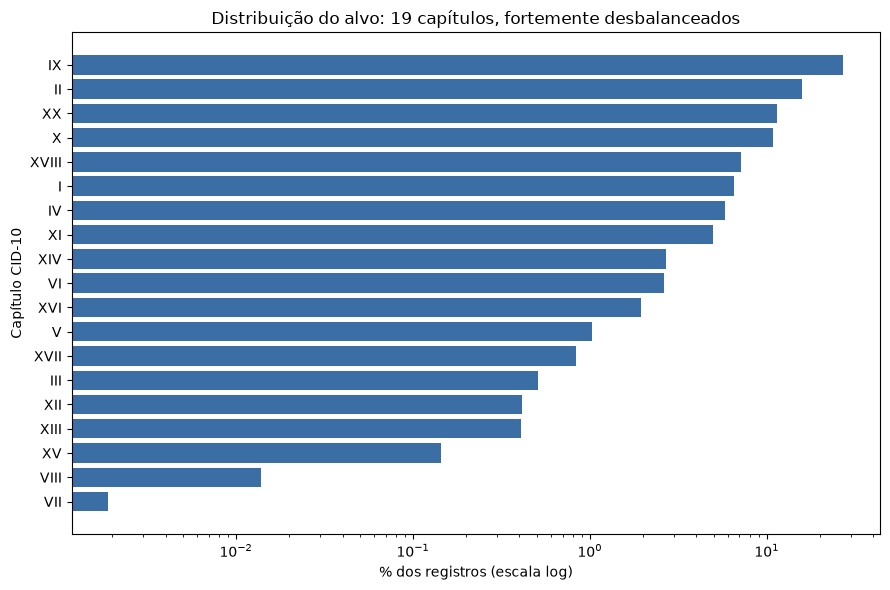
\includegraphics[width=0.85\textwidth]{figuras/distribuicao_capitulos.png}
\caption{Participação de cada capítulo da CID-10 no total de registros, em
  escala logarítmica. Os capítulos XIX e XXI não aparecem porque nunca ocorrem
  como causa básica nesta base.}
\label{fig:distribuicao}
\end{figure}

\section{Resultados Parciais}
\label{sec:resultados}

\subsection{Aspectos éticos e responsabilidade no uso da IA}
\label{sec:etica}

O projeto usa exclusivamente os microdados públicos do SIM, publicados como dados abertos pelo Ministério da Saúde sob licença CC-BY, e os utiliza como foram disponibilizados. Das 8 colunas lidas, nenhuma é identificador direto (nome, CPF, endereço). A Lei Geral de Proteção
de Dados Pessoais~\cite{lgpd} define dado anonimizado como aquele ``relativo a titular que não possa ser identificado, considerando a utilização de meios técnicos razoáveis e disponíveis na ocasião de seu tratamento'' (art.~5º, inciso III) e estabelece, no art.~12, que dados anonimizados não são considerados dados pessoais, \emph{salvo} quando a anonimização puder ser revertida com esforços razoáveis. É exatamente essa ressalva que nos obriga a ter cuidado: a combinação de quase-identificadores (idade, município de residência e data do óbito) pode permitir reidentificação por inferência em municípios pequenos ou para causas raras.

Um modelo que ``acertasse'' a causa porque leu a descrição da causa não mediria associação nenhuma, e reportá-lo como resultado seria enganoso. A prevenção estrutural e verificada em código descrita na Seção~\ref{sec:metodologia} é, portanto, também uma exigência de honestidade na apresentação dos resultados.

O não-preenchimento de \texttt{RACACOR} e \texttt{ESC} é grande e muda muito ao longo dos anos (Figura~\ref{fig:ausentes}). Um modelo treinado sobre esses dados herda qualquer padrão sistemático desse não-preenchimento, por exemplo, se a ausência for mais comum em certos
serviços de saúde ou regiões, algo que não medimos. Por isso mantemos
``Ignorado'' como categoria explícita em vez de imputar valores, o que
esconderia o viés em vez de expô-lo. Reconhecemos como limitação que ainda não realizamos análise de erro por subgrupo (raça/cor, sexo, UF), prevista para a etapa seguinte do projeto.

O objetivo é apoiar o planejamento em saúde pública em nível agregado. O modelo não deve ser usado para decisões individuais sobre pessoas vivas, nem para inferir a causa de uma morte específica sem o laudo médico, que é a fonte de verdade. O desempenho absoluto medido (Seção~\ref{sec:desempenho}) reforça essa restrição: um F1-macro em
torno de 0,14 é incompatível com qualquer uso individual.

O alvo é o capítulo da CID-10, e não o código completo. Além de evitar centenas de classes, isso produz uma categoria ampla e auditável, que reduz o risco de decisões automatizadas granulares e mal calibradas a partir de poucas variáveis sociodemográficas. Todo o código, incluindo a preparação e as asserções de ausência de vazamento, é público.

O projeto usa exclusivamente dados públicos, secundários e anonimizados, sem acesso a registros identificáveis, sem vinculação com outras bases e sem contato com pessoas. Por esses critérios, e em linha com a orientação da disciplina, o grupo conclui que, em princípio, a submissão ao CEP não é necessária. Isso mudaria se o projeto passasse a usar registros identificáveis ou de acesso restrito, cruzasse o SIM com outra base ou envolvesse contato direto com pessoas; nenhuma dessas condições se aplica hoje, e, se alguma passar a valer, a necessidade de submissão deve ser reavaliada antes de prosseguir.

\subsection{Detalhamento dos resultados parciais}
\label{sec:desempenho}

Os três modelos foram treinados sobre as 26.025.534 linhas de treino
\emph{completas}, sem subamostragem, e avaliados sobre as mesmas 6.506.384 linhas de teste, em um servidor Linux, com treino paralelizado em todos os núcleos disponíveis (\texttt{n\_jobs = -1}). As configurações são iniciais e nenhum hiperparâmetro foi ajustado: baseline de classe majoritária; Random Forest com 100 árvores e profundidade máxima 12; XGBoost com 100 rodadas, profundidade 6, taxa de aprendizado 0,3 e \texttt{tree\_method = "hist"}. Os dois modelos receberam os mesmos pesos de amostra balanceados.

\begin{table}[ht]
\centering
\caption{Comparação dos três modelos no conjunto de teste (6.506.384 linhas,
  divisão estratificada 80/20). A acurácia consta apenas como referência.}
\label{tab:comparacao}
\small
\begin{tabular}{|l|r|r|r|r|}
\hline
\textbf{Modelo} & \textbf{F1-macro} & \textbf{Acurácia} & \textbf{Recall macro}
  & \textbf{Tempo de treino} \\
\hline
Baseline (classe majoritária) & 0,0224 & 0,2701 & 0,0526 &     3,1 s \\
Random Forest                 & 0,1329 & 0,1625 & 0,2234 &   343,9 s \\
XGBoost                       & \textbf{0,1406} & 0,1755 & 0,2294 &   983,3 s \\
\hline
\end{tabular}
\end{table}

Em F1-macro, o Random Forest supera o baseline em $+0{,}1105$ (5,9 vezes) e o XGBoost em $+0{,}1183$ (6,3 vezes). Os dois modelos também superam o baseline em recall macro (0,2234 e 0,2294 contra 0,0526). Em acurácia, porém, o baseline vence (0,2701 contra 0,1625 e 0,1755). Esse resultado não é um defeito, e sim a consequência direta e prevista dos pesos balanceados: o baseline atinge 27\% de acurácia prevendo sempre o capítulo IX e errando todas as outras 18 classes, enquanto os modelos
ponderados distribuem suas predições entre as classes e abrem mão dos acertos fáceis na classe majoritária. É precisamente por isso que a acurácia não é o critério deste trabalho.

O XGBoost obteve F1-macro 0,0078 maior (cerca de 6\% em termos relativos) gastando 983,3 s contra 343,9 s de treino, ou seja, 2,86 vezes mais tempo. Na checagem temporal a razão foi ainda maior (1.322,3 s contra 352,9 s). O ganho aparece em alguns capítulos (II: 0,2473 contra 0,1765; XIV: 0,1022 contra 0,0593; IX: 0,0260 contra 0,0013) e se inverte em outros (XVI: 0,8602 contra 0,8373; XX: 0,5363 contra 0,4975; XIII: 0,0886 contra 0,0454). Como as duas configurações iniciais têm profundidades diferentes (12 e 6) e nenhuma foi ajustada, esta comparação não mostra qual família é superior após ajuste fino. Nossa leitura, para o estágio atual: o Random Forest é a opção mais barata e chega perto; o XGBoost passa a valer o custo se o ajuste de hiperparâmetros ampliar a vantagem, o que ainda precisa ser verificado.

Treinando com 2000-2022 (27.506.105 linhas) e testando em anos não vistos
(Tabela~\ref{tab:temporal}), o F1-macro cai de forma leve e monótona: 0,0051 do Random Forest e 0,0053 do XGBoost entre 2023 e 2026. O F1-macro agregado do teste temporal fica cerca de 0,01 abaixo do protocolo principal. Essa comparação, porém, não isola a deriva temporal, porque o conjunto de treino tem outro tamanho e o de teste é um conjunto diferente de anos, com outra mistura de classes; o baseline não foi recalculado nessa checagem. A mudança na qualidade do preenchimento ao longo dos anos é uma explicação possível para a deriva, mas não foi testada. O ano de 2026 é parcial (506.027 linhas contra 1.463.485 em 2023), o que torna seu F1-macro menos estável.

\begin{table}[ht]
\centering
\caption{Checagem suplementar de generalização temporal: treino com 2000--2022,
  teste em anos não vistos. F1-macro.}
\label{tab:temporal}
\begin{tabular}{|l|r|r|r|r|}
\hline
\textbf{Modelo} & \textbf{2023} & \textbf{2025} & \textbf{2026 (parcial)}
  & \textbf{Agregado} \\
\hline
Random Forest & 0,1253 & 0,1216 & 0,1202 & 0,1230 \\
XGBoost       & 0,1340 & 0,1297 & 0,1287 & 0,1314 \\
\hline
\end{tabular}
\end{table}

O resultado principal é que o desempenho absoluto é baixo: um F1-macro de 0,13 a 0,14 significa que a maioria dos 19 capítulos é reconhecida de forma fraca. O ganho sobre o baseline é real e grande em termos relativos, e mostra que os modelos aprenderam algo, mas o que eles aprenderam é, essencialmente, o efeito de idade e sexo sobre um punhado de capítulos. Nossa interpretação é que cinco atributos sociodemográficos carregam pouco sinal sobre a categoria da causa básica de óbito, o que é em si uma informação relevante: a maior parte dos óbitos ocorre em adultos e idosos, faixa em que os capítulos principais (circulatório, neoplasias, respiratório, endócrino) competem dentro do mesmo perfil demográfico. Não apresentamos esses números como um classificador utilizável, e sim como a medida de um limite.

\subsection{Limitações e próximos passos (N2)}

As limitações reconhecidas são: (i) uma única divisão e uma única semente, sem intervalos de confiança; (ii) hiperparâmetros não ajustados, com profundidades diferentes entre os dois modelos; (iii) conclusões sobre os capítulos VII e VIII apoiadas em 126 e 898 casos de teste; (iv) ausência de análise de erro por subgrupo; (v) a decisão de mapear o código 0 de \texttt{ESC} para ``Ignorado'', que pode significar ``nenhuma escolaridade''; e (vi) a política de supressão de células com menos de 10 casos ainda não implementada em código.

Para o segundo bimestre, os caminhos previstos são: ajuste de hiperparâmetros dos dois modelos sob o mesmo protocolo; avaliação de atributos adicionais que comprovadamente não vazem o rótulo; inclusão de variáveis temporais, como mês e ano do óbito; variáveis agregadas em nível de município com granularidade suficiente para respeitar a supressão de grupos pequenos; e análise de erro por subgrupo, para avaliar equidade. A expectativa, dado o que foi medido aqui, é de ganhos moderados: o limite observado parece vir do conjunto de atributos, não da escolha do algoritmo.

\subsection{Endereço do repositório no GitHub}

Todo o material do projeto está em um repositório público:
\url{https://github.com/araujoviana/projeto1-IA-2026}. Ele contém este artigo
(fontes LaTeX e PDF), a descrição do dataset e o procedimento para obtê-lo
(\texttt{data/README.md}, sem os microdados brutos, que são um download
público de grande porte), os três notebooks Python executados com seus
resultados (\texttt{notebooks/}), o módulo de funções com testes
automatizados (\texttt{src/} e \texttt{tests/}) e o histórico completo de
alterações no Git. 

\section{Referências}

\bibliographystyle{sbc}
\bibliography{referencias}

\end{document}
